\documentclass{standalone}

\begin{document}

\section[CHIMeRA as Service]{CHIMeRA as Service}\label{chimera:caas}

We have discussed about the informations stored into the \textsf{CHIMeRA} database but we have ignored how we could manage these data.
More than the realization of a useful database we have to provide an easy-to-use interface to encourage the research community to manage our processed informations.
We have already talked about how the modern databases are shared in Internet and how these large quantities of data could be managed using database languages (ref. \ref{chimera:chimera}).
Now we have to find the best solution for our application.

We developed a first database version of \textsf{CHIMeRA} using \textsf{SQLite} language.
\textsf{SQLite} language is probably the easier solution for database management and the realization of efficient query is straightforward.
It is a well performing solution for standard relational databases but it does not provide any facility for network structure.
Moreover, \textsf{SQLite} database is hard to share along the Internet: the language supports the port forwarding connection but it is not easy to set read/write privileges like using other solutions like \textsf{MySQL} one.

A more efficient solution is provided by the modern graph databases (GDB).
GDB are databases which use graph structures to represent and store informations: there are two needed informations for the database given by nodes and edges.
The key concept behind this kind of storage is the relationship between the entries and they go under the \textsf{NoSQL} database category.
GDBs allow simple and efficient retrieval of complex hierarchical structures by definition and thus they represent the most efficient solution for our \textsf{CHIMeRA} database which is born as network-of-networks.
Multiple different solutions have been proposed to address graphs storage and there are a wide range of possible GDB languages public available on-line (e.g \textsf{Neo4j}, \textsf{OrientDB}, \textsf{Sparksee}, \textsf{AllegroGraph}, $\cdots$).
Based on our experience about these topics and driven by the available documentation, we have chosen to use \href{https://www.arangodb.com/}{\textsf{ArangoDB}} in our application.
\textsf{ArangoDB} is an open-source and free software released on Github for multi-model database management with a unified query language \textsf{AQL} (\emph{ArangoDB Query Language}).
\textsf{ArangoDB} database system is \textsf{NoSQL} but its queries are very closed to \textsf{SQL} ones and thus are easier to write also by no-expert users.
The core is written in \textsf{C++} and thus extremely efficient from a numerical point-of-view.
Moreover, it provides also a user-friendly web interface for network visualization and queries.
The possibility to have a web interface allows an easy way to share our database on Internet as service increasing the usability of our tool.
Moreover the query outputs can be also downloaded and used by external tools.
Thus, using \textsf{ArangoDB} as service management we can provide a \emph{Software as a Service} (SaaS) interface of our \textsf{CHIMeRA} database.
This project is still in work in progress and this SaaS is not yet public available\footnote{
  As soon as possible we intend to create it jointly to an adequate computational environment able to support multiple external queries.
}.

We re-formatted the \textsf{CHIMeRA} network following the \textsf{ArangoDB} requirements and we create the graph database structure of our data.
Using this database we were able to perform the first queries and discuss about the results.
In particular, we focused on two entries of our database which are interesting topics for the research group: the \emph{leukemia} disease and the \emph{PRNP} gene.
We customized our query to extract only the 2-order connections related to these nodes.
The pseudo-code used for our queries is showed in \ref{code:query}.

\lstset{style=Java}
\begin{lstlisting}[language=Java, caption=CHIMeRA 2-order connections query, label=code:query]
FOR x IN node_type_vertex
  FILTER x.name LIKE "looking_for_entry"
    FOR v, e, p IN 1..3 ANY x GRAPH "CHIMeRA"
      RETURN p
\end{lstlisting}

The query takes the node-collection (\textsf{ArangoDB} nomenclature) related to the searched node type (\textsf{node\_type\_vertex} in the code) and filter all the name which satisfy the \textsf{LIKE} condition.
Starting from the founded nodes it returns the output graph preview made by the 1st and 2nd order connections (range of values \textsf{1..3} in the code).

We applied this kind of query for the two nodes and we processed the results using \textsf{Gephi} as network viewer.
The obtained results are showed in Fig.\ref{fig:leukemia} and Fig.\ref{fig:prnp} for the \emph{leukemia} (\numprint{9460} nodes and \numprint{26646} links) and \emph{PRNP} (\numprint{19103} nodes and \numprint{139496} links) queries, respectively.
As can be seen by the two figures, both networks are quite large just considering the 2-order connections and they highlight the biological complexity of these entries.

\begin{figure}[htbp]
\centering
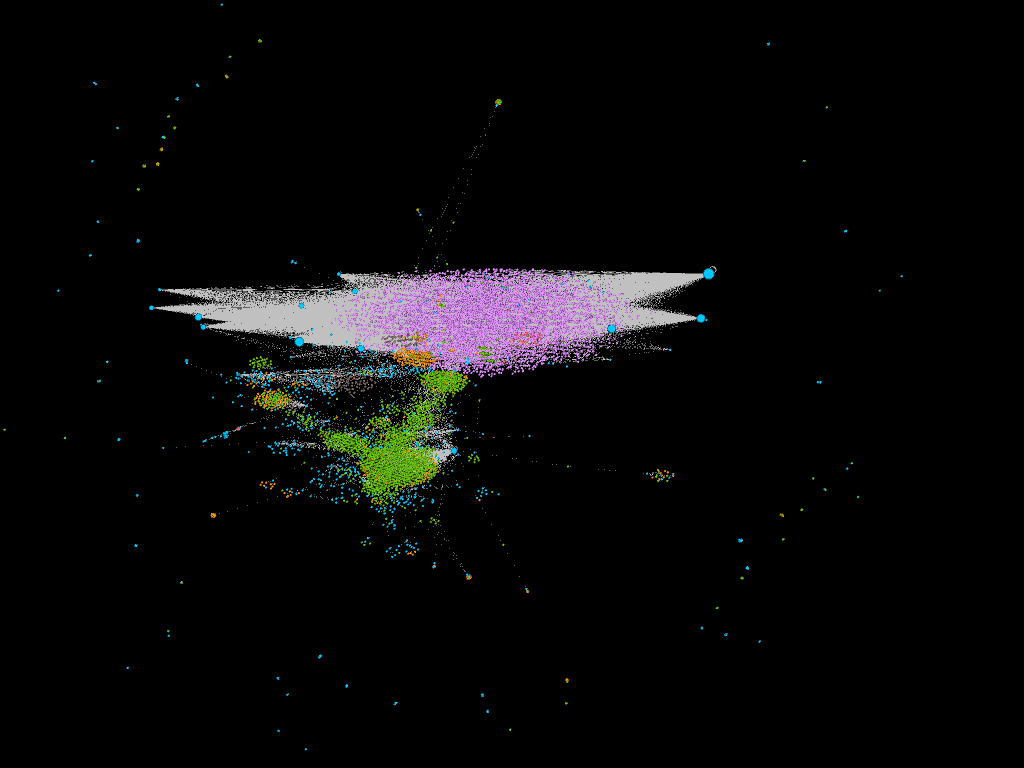
\includegraphics[width=.8\linewidth]{leukemia.png}
\caption{Output of \emph{leukemia} query obtained by \textsf{CHIMeRA} graph database using \ref{code:query}.
The subnetwork is made by the 2-order connections starting from all the nodes which include \quotes{leukemia} in their names.
The subnetwork includes 291 different types of leukemias clustered into 82 connected components.
The giant components is made by \numprint{9108} nodes.
\textsf{CHIMeRA} query is able to give a panoramic biomedical overview of the \emph{leukemia} diseases mapping 838 diseases, \numprint{2463} genes, 5195 SNPs, 154 metabolite pathways, 40 metabolites and 5 drugs associated to them.
}
\label{fig:leukemia}
\end{figure}

\begin{figure}[htbp]
\centering
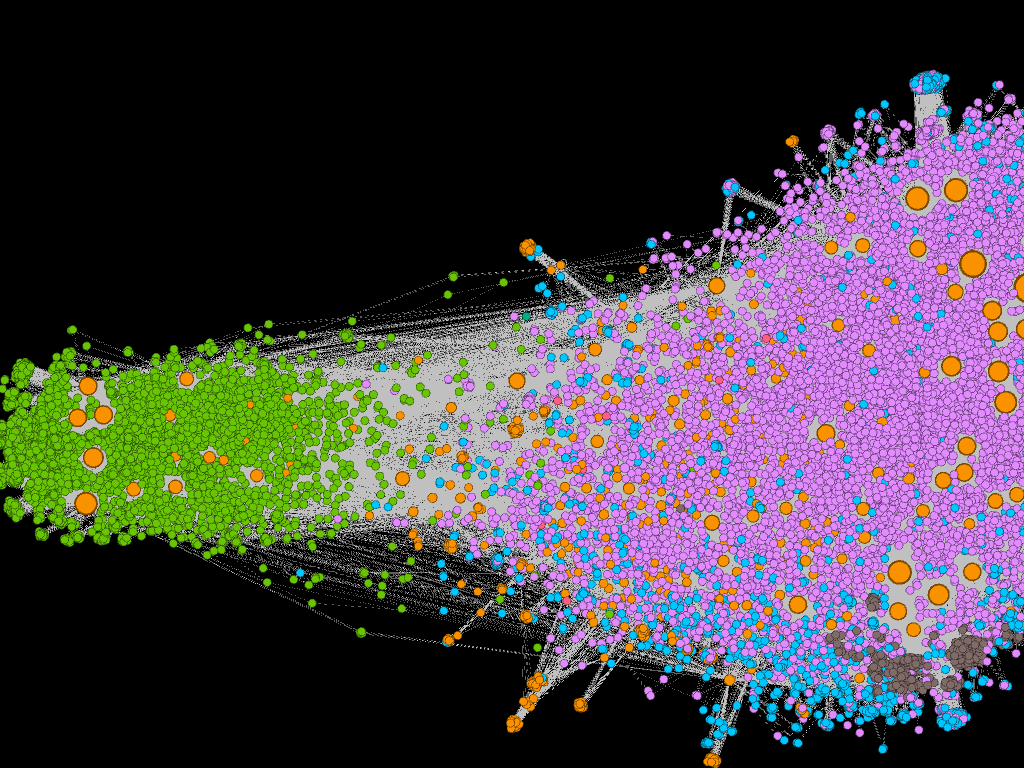
\includegraphics[width=.8\linewidth]{PRNP.png}
\caption{Output of \emph{PRNP} query obtained by \textsf{CHIMeRa} graph database using \ref{code:query}.
The subnetwork is made by the 2-order connections starting from the \emph{PRNP} gene node and it includes \numprint{19103} nodes and \numprint{139496} links.
The subnetwork highlights the connections of \emph{PRNP} gene to 777 diseases, 9 drugs, \numprint{10452} genes, 1 metabolite, 576 metabolite pathways, \numprint{3775} phenotypes and \numprint{3513} SNPs.
}
\label{fig:prnp}
\end{figure}

Using the \quotes{generic} name of \emph{leukemia} we found 291 different types of leukemia diseases into the \textsf{CHIMeRA} database which denote the different facets of the disease.
Despite these multiplicities of results, we noticed that they clustered in only 82 connected components highlighting multiple similitudes between them.
In particular we found a giant components of \numprint{9108} nodes and only other 6 components with more than 10 nodes.
This result highlights that despite we have multiple informations about some leukemia types we are still missing an heterogeneous overview of some critical cases.
The powerful of \textsf{CHIMeRA} network born exactly from these cases, in which we can infer missing informations starting from the knowledge about analogous researches given by the full set of informations related to the giant component found.
The subnetwork extracted, in fact, as multiple node types which enrich the biomedical description of the leukemia diseases: we found 838 diseases, \numprint{2463} genes, 5195 SNPs, 154 metabolite pathways, 40 metabolites and 5 drugs associated to the different kind of leukemias.
A such biomedical panoramic overview could not be found using a single-database approach and, to the best of the author's knowledge, only the \textsf{CHIMeRA} structure is capable to map them.

A comparable informative result is found looking for the \emph{PRNP} gene in which only 1 connected component is found (as expected).
Also in this case the \textsf{CHIMeRA} network is able to associate to the gene multiple information types (777 diseases, 9 drugs, \numprint{10452} genes, 1 metabolite, 576 metabolite pathways, \numprint{3775} phenotypes and \numprint{3513} SNPs).

We are still working on the analyses of the extracted informations and especially on their biomedical interpretation.
Thus, we conclude this chapter remarking the potential applications of such network-of-networks structure and its capability of give us a more global overview of biomedical compounds in scientific researches.

\end{document}
